\documentclass[10pt]{article}\usepackage[]{graphicx}\usepackage[]{color}
%% maxwidth is the original width if it is less than linewidth
%% otherwise use linewidth (to make sure the graphics do not exceed the margin)
\makeatletter
\def\maxwidth{ %
  \ifdim\Gin@nat@width>\linewidth
    \linewidth
  \else
    \Gin@nat@width
  \fi
}
\makeatother

\definecolor{fgcolor}{rgb}{0.345, 0.345, 0.345}
\newcommand{\hlnum}[1]{\textcolor[rgb]{0.686,0.059,0.569}{#1}}%
\newcommand{\hlstr}[1]{\textcolor[rgb]{0.192,0.494,0.8}{#1}}%
\newcommand{\hlcom}[1]{\textcolor[rgb]{0.678,0.584,0.686}{\textit{#1}}}%
\newcommand{\hlopt}[1]{\textcolor[rgb]{0,0,0}{#1}}%
\newcommand{\hlstd}[1]{\textcolor[rgb]{0.345,0.345,0.345}{#1}}%
\newcommand{\hlkwa}[1]{\textcolor[rgb]{0.161,0.373,0.58}{\textbf{#1}}}%
\newcommand{\hlkwb}[1]{\textcolor[rgb]{0.69,0.353,0.396}{#1}}%
\newcommand{\hlkwc}[1]{\textcolor[rgb]{0.333,0.667,0.333}{#1}}%
\newcommand{\hlkwd}[1]{\textcolor[rgb]{0.737,0.353,0.396}{\textbf{#1}}}%
\let\hlipl\hlkwb

\usepackage{framed}
\makeatletter
\newenvironment{kframe}{%
 \def\at@end@of@kframe{}%
 \ifinner\ifhmode%
  \def\at@end@of@kframe{\end{minipage}}%
  \begin{minipage}{\columnwidth}%
 \fi\fi%
 \def\FrameCommand##1{\hskip\@totalleftmargin \hskip-\fboxsep
 \colorbox{shadecolor}{##1}\hskip-\fboxsep
     % There is no \\@totalrightmargin, so:
     \hskip-\linewidth \hskip-\@totalleftmargin \hskip\columnwidth}%
 \MakeFramed {\advance\hsize-\width
   \@totalleftmargin\z@ \linewidth\hsize
   \@setminipage}}%
 {\par\unskip\endMakeFramed%
 \at@end@of@kframe}
\makeatother

\definecolor{shadecolor}{rgb}{.97, .97, .97}
\definecolor{messagecolor}{rgb}{0, 0, 0}
\definecolor{warningcolor}{rgb}{1, 0, 1}
\definecolor{errorcolor}{rgb}{1, 0, 0}
\newenvironment{knitrout}{}{} % an empty environment to be redefined in TeX

\usepackage{alltt}

\usepackage{amsmath,amssymb,amsthm}
\usepackage{fancyhdr,url,hyperref}
\usepackage{graphicx,xspace}
\usepackage{subfigure}
\usepackage{tikz}
\usetikzlibrary{arrows,decorations.pathmorphing,backgrounds,positioning,fit,through}

\oddsidemargin 0in  %0.5in
\topmargin     0in
\leftmargin    0in
\rightmargin   0in
\textheight    9in
\textwidth     6in %6in
\setlength{\parindent}{0in}
%\headheight    0in
%\headsep       0in
%\footskip      0.5in

\newtheorem{thm}{Theorem}
\newtheorem{cor}[thm]{Corollary}
\newtheorem{obs}{Observation}
\newtheorem{lemma}{Lemma}
\newtheorem{claim}{Claim}
\newtheorem{definition}{Definition}
\newtheorem{question}{Question}
\newtheorem{answer}{Answer}
\newtheorem{problem}{Problem}
\newtheorem{solution}{Solution}
\newtheorem{conjecture}{Conjecture}

\pagestyle{fancy}

\lhead{\textsc{Prof. McNamara}}
\chead{\textsc{SDS/MTH 220: Lecture notes}}
\lfoot{}
\cfoot{}
%\cfoot{\thepage}
\rfoot{}
\renewcommand{\headrulewidth}{0.2pt}
\renewcommand{\footrulewidth}{0.0pt}

\newcommand{\ans}{\vspace{0.25in}}
\newcommand{\R}{{\sf R}\xspace}
\newcommand{\cmd}[1]{\texttt{#1}}
\newcommand{\Ex}{\mathbb{E}}

\rhead{\textsc{November 3, 2017}}
\IfFileExists{upquote.sty}{\usepackage{upquote}}{}
\begin{document}

\paragraph{Agenda}
\begin{enumerate}
  \itemsep0em
  \item Inference for a single proportion
\end{enumerate}




%   \item \textbf{Blackjack} In blackjack, you are dealt two cards, and all face cards count as 10. The ace can be one or eleven. What is the expected value of a randomly dealt hand from an infinite shoe? What is the probability of being dealt at least a 20? 
% 
% 
% \begin{proof}
%   Let $X_1, X_2$ be r.v. for the value of the two cards. Then since the shoe is infinite, $\Ex[X_1] = \Ex[X_2]$. Assuming that aces are always worth one, we have:
%   $$
%     \Ex[X_i] = \frac{1}{13} \left( \sum_{i=1}^9 i + 4 \cdot 10 \right) = \frac{1}{13} \left( \binom{10}{2} + 40 \right) = \frac{45 + 40}{13} = \frac{85}{13} \approx 6.5
%   $$
%   So then $\Ex[X_1 + X_2] \approx 13$. Allowing aces to be more than one improves this slightly. 
%   
%   There are $13 \cdot 13 = 169$ possible pairs. There are $4^2 = 16$ ways to get 20 without an ace. There are $2 \cdot 4 = 8$ ways to get blackjack. There are two ways to get 20 with an ace and a 9. Thus, there are $16 + 8 + 2 = 26$ ways to get at least a 20. Thus, the probability $\Pr[X_1 + X_2 \geq 20] = \frac{26}{169} \approx 15.4$\%. 
% \end{proof}


\paragraph{Inference for a Single Proportion}

% Beware the \href{http://en.wikipedia.org/wiki/Law_of_the_instrument}{Law of the Instrument}:
% 
% \begin{quotation}
%   If all you have is a hammer, everything looks like a nail.\\
%   --Abraham Maslow, \textit{The Psychology of Science}
% \end{quotation}

Consider the following problem: In a survey of a simple random sample of 123 people 77 say they prefer Coke over Pepsi. Then a point estimate for the proportion of people who prefer Coke over Pepsi is $\hat{p} =77/123 = 0.624$.

In order to make inferences about the unknown value of $p$, the true proportion of those in population who prefer Coke, we have to construct the sampling distribution of $\hat{p}$. The center, shape, and spread of the sampling distribution of the proportion will enable us to put the observed $\hat{p}$ in context, build confidence intervals, and conduct hypothesis tests. 

There are at least three different ways to approximate the sampling distribution of $\hat{p}$:

\begin{enumerate}
  \item Simulation: This is one of the central themes of this course. For example, to test the null hypothesis that $p_0 = 0.5$, we simulate many random draws from this distribution, and see where $\hat{p}$ lies in this simulated distribution. 
  
  
\begin{knitrout}
\definecolor{shadecolor}{rgb}{0.969, 0.969, 0.969}\color{fgcolor}\begin{kframe}
\begin{alltt}
\hlstd{n} \hlkwb{<-} \hlnum{123}
\hlstd{p_0} \hlkwb{<-} \hlnum{1}\hlopt{/}\hlnum{2}
\hlstd{p_hat} \hlkwb{<-} \hlnum{77}\hlopt{/}\hlnum{123}
\hlkwd{library}\hlstd{(mosaic)}
\hlkwd{library}\hlstd{(oilabs)}
\hlstd{outcomes} \hlkwb{<-} \hlkwd{data_frame}\hlstd{(}\hlkwc{soda} \hlstd{=} \hlkwd{c}\hlstd{(}\hlstr{"Coke"}\hlstd{,} \hlstr{"Pepsi"}\hlstd{))}
\hlstd{sim} \hlkwb{<-} \hlstd{outcomes} \hlopt
  \hlkwd{rep_sample_n}\hlstd{(}\hlkwc{size} \hlstd{= n,} \hlkwc{replace} \hlstd{=} \hlnum{TRUE}\hlstd{,} \hlkwc{reps} \hlstd{=} \hlnum{10000}\hlstd{)} \hlopt
  \hlkwd{group_by}\hlstd{(replicate)} \hlopt
  \hlkwd{summarize}\hlstd{(}\hlkwc{N} \hlstd{=} \hlkwd{n}\hlstd{(),} \hlkwc{coke} \hlstd{=} \hlkwd{sum}\hlstd{(soda} \hlopt{==} \hlstr{"Coke"}\hlstd{))} \hlopt
  \hlkwd{mutate}\hlstd{(}\hlkwc{coke_pct} \hlstd{= coke} \hlopt{/} \hlstd{N)}
\hlkwd{qplot}\hlstd{(}\hlkwc{data} \hlstd{= sim,} \hlkwc{x} \hlstd{= coke_pct,} \hlkwc{geom} \hlstd{=} \hlstr{"density"}\hlstd{)}
\end{alltt}
\end{kframe}
\end{knitrout}

It is important to recognize that by drawing more and more samples, we get a more refined understanding of the sampling distribution, but it remains only an approximation. 
  
The p-value can be obtained using the \cmd{pdata} function, since the sampling distribution comes from simulated data in our workspace.

\begin{knitrout}
\definecolor{shadecolor}{rgb}{0.969, 0.969, 0.969}\color{fgcolor}\begin{kframe}
\begin{alltt}
\hlnum{2} \hlopt{*} \hlkwd{pdata}\hlstd{(}\hlopt{~} \hlstd{coke_pct,} \hlkwc{q} \hlstd{= p_hat,} \hlkwc{data} \hlstd{= sim,} \hlkwc{lower.tail} \hlstd{=} \hlnum{FALSE}\hlstd{)}
\end{alltt}
\begin{verbatim}
## [1] 0.0052
\end{verbatim}
\end{kframe}
\end{knitrout}
  
 \begin{enumerate}
    \item Assumptions: independence
    \item Pros: few assumptions, no math, can simulate very complex situations with a little programming skill
    \item Cons: requires computer (impossible before 1970), does not always return the same answer
  \end{enumerate}  
  
\clearpage  
\item Probability Theory: If we assume that each person's preference is independent, and the that the true proportion is fixed, then the number of individuals who will say that they prefer Coke is a random variable that follows a \emph{binomial} distribution. 

\vfill


  
\begin{knitrout}
\definecolor{shadecolor}{rgb}{0.969, 0.969, 0.969}\color{fgcolor}\begin{kframe}
\begin{alltt}
\hlkwd{plotDist}\hlstd{(}\hlstr{"binom"}\hlstd{,} \hlkwc{params} \hlstd{=} \hlkwd{list}\hlstd{(}\hlkwc{size} \hlstd{= n,} \hlkwc{prob} \hlstd{= p_0))}
\end{alltt}
\end{kframe}
\end{knitrout}

The p-value can be obtained using the \cmd{pbinom} function, since the sampling distribution follows a binomial distribution.

\begin{knitrout}
\definecolor{shadecolor}{rgb}{0.969, 0.969, 0.969}\color{fgcolor}\begin{kframe}
\begin{alltt}
\hlnum{2} \hlopt{*} \hlkwd{pbinom}\hlstd{(p_hat} \hlopt{*} \hlstd{n,} \hlkwc{size} \hlstd{= n,} \hlkwc{prob} \hlstd{= p_0,} \hlkwc{lower.tail} \hlstd{=} \hlnum{FALSE}\hlstd{)}
\end{alltt}
\begin{verbatim}
## [1] 0.003731446
\end{verbatim}
\end{kframe}
\end{knitrout}

The binomial distribution depends on two parameters: the sample size $n$ and the proportion $p$. We won't talk much more about the binomial distribution in this class (to learn more, take MTH 153 or MTH 246). 
.
  \begin{enumerate}
    \item Assumptions: independence, probability model
    \item Pros: gives exact sampling distribution
    \item Cons: only the simplest situations can be solved in closed form, may be hard to detect mistakes
  \end{enumerate}
  
\clearpage
\item Normal Approximation: Since the binomial distribution can be cumbersome to work with, and because under very mild conditions it is approximately normal, statisticians most often use a normal distribution to approximate the sampling distribution for a single proportion. If the number of individuals who prefer Coke follows a binomial distribution with parameters $n$ and $p$, then it follows from elementary probability theory that the standard deviation of the proportion who prefer Coke is $SE_{\hat{p}} = \sqrt{\frac{\hat{p}(1-\hat{p})}{n}}$. Thus, we can use this formula for the standard error to estimate the sampling distribution and conduct our hypothesis test.
  
\begin{knitrout}
\definecolor{shadecolor}{rgb}{0.969, 0.969, 0.969}\color{fgcolor}\begin{kframe}
\begin{alltt}
\hlstd{se_p} \hlkwb{<-} \hlkwd{sqrt}\hlstd{(p_0} \hlopt{*} \hlstd{(}\hlnum{1}\hlopt{-}\hlstd{p_0)} \hlopt{/} \hlstd{n)}
\hlkwd{plotDist}\hlstd{(}\hlstr{"norm"}\hlstd{,} \hlkwc{params} \hlstd{=} \hlkwd{list}\hlstd{(}\hlkwc{mean} \hlstd{= p_0,} \hlkwc{sd} \hlstd{= se_p))}
\end{alltt}
\end{kframe}
\end{knitrout}

  The p-value can be obtained using the \cmd{pnorm} function, since the sampling distribution follows a normal distribution.

\begin{knitrout}
\definecolor{shadecolor}{rgb}{0.969, 0.969, 0.969}\color{fgcolor}\begin{kframe}
\begin{alltt}
\hlnum{2} \hlopt{*} \hlkwd{pnorm}\hlstd{(p_hat,} \hlkwc{mean} \hlstd{= p_0,} \hlkwc{sd} \hlstd{= se_p,} \hlkwc{lower.tail} \hlstd{=} \hlnum{FALSE}\hlstd{)}
\end{alltt}
\begin{verbatim}
## [1] 0.005187149
\end{verbatim}
\end{kframe}
\end{knitrout}

For a variety of reasons both historical and practical, the normal approximation is the method you are mostly likely to see in your future work, and thus it will be the focus of our attention here. 

 \begin{enumerate}
    \item Assumptions: independence, normality, $np > 10$ and $n(1-p) > 10$
    \item Pros: uses familiar normal distribution, approximation is usually pretty good, possible to compute without computers (kind of)
    \item Cons: requires more assumptions, not exact
  \end{enumerate}

\end{enumerate}

Note that the p-value is slightly different in each case (since our approximation of the sampling distribution is different in each case), but it is very close, and in each case we will easily reject the null hypothesis that $p = 0.5$ at the 5\% level. 

\paragraph{What Can Go Wrong?}

Most of the time, the sampling distribution for a proportion will be quite normal. In the previous example, the fit was excellent.




\begin{knitrout}
\definecolor{shadecolor}{rgb}{0.969, 0.969, 0.969}\color{fgcolor}\begin{kframe}
\begin{alltt}
\hlkwd{qplot}\hlstd{(}\hlkwc{data} \hlstd{= sim,} \hlkwc{x} \hlstd{= coke_pct,} \hlkwc{geom} \hlstd{=} \hlstr{"density"}\hlstd{)} \hlopt{+}
  \hlkwd{stat_function}\hlstd{(}\hlkwc{fun} \hlstd{= dbinom_p,} \hlkwc{args} \hlstd{=} \hlkwd{c}\hlstd{(}\hlkwc{size} \hlstd{= n,} \hlkwc{prob} \hlstd{= p_0),} \hlkwc{col} \hlstd{=} \hlstr{"red"}\hlstd{)} \hlopt{+}
  \hlkwd{stat_function}\hlstd{(}\hlkwc{fun} \hlstd{= dnorm,} \hlkwc{args} \hlstd{=} \hlkwd{c}\hlstd{(}\hlkwc{mean} \hlstd{= p_0,} \hlkwc{sd} \hlstd{= se_p),} \hlkwc{col} \hlstd{=} \hlstr{"purple"}\hlstd{)}
\end{alltt}
\end{kframe}
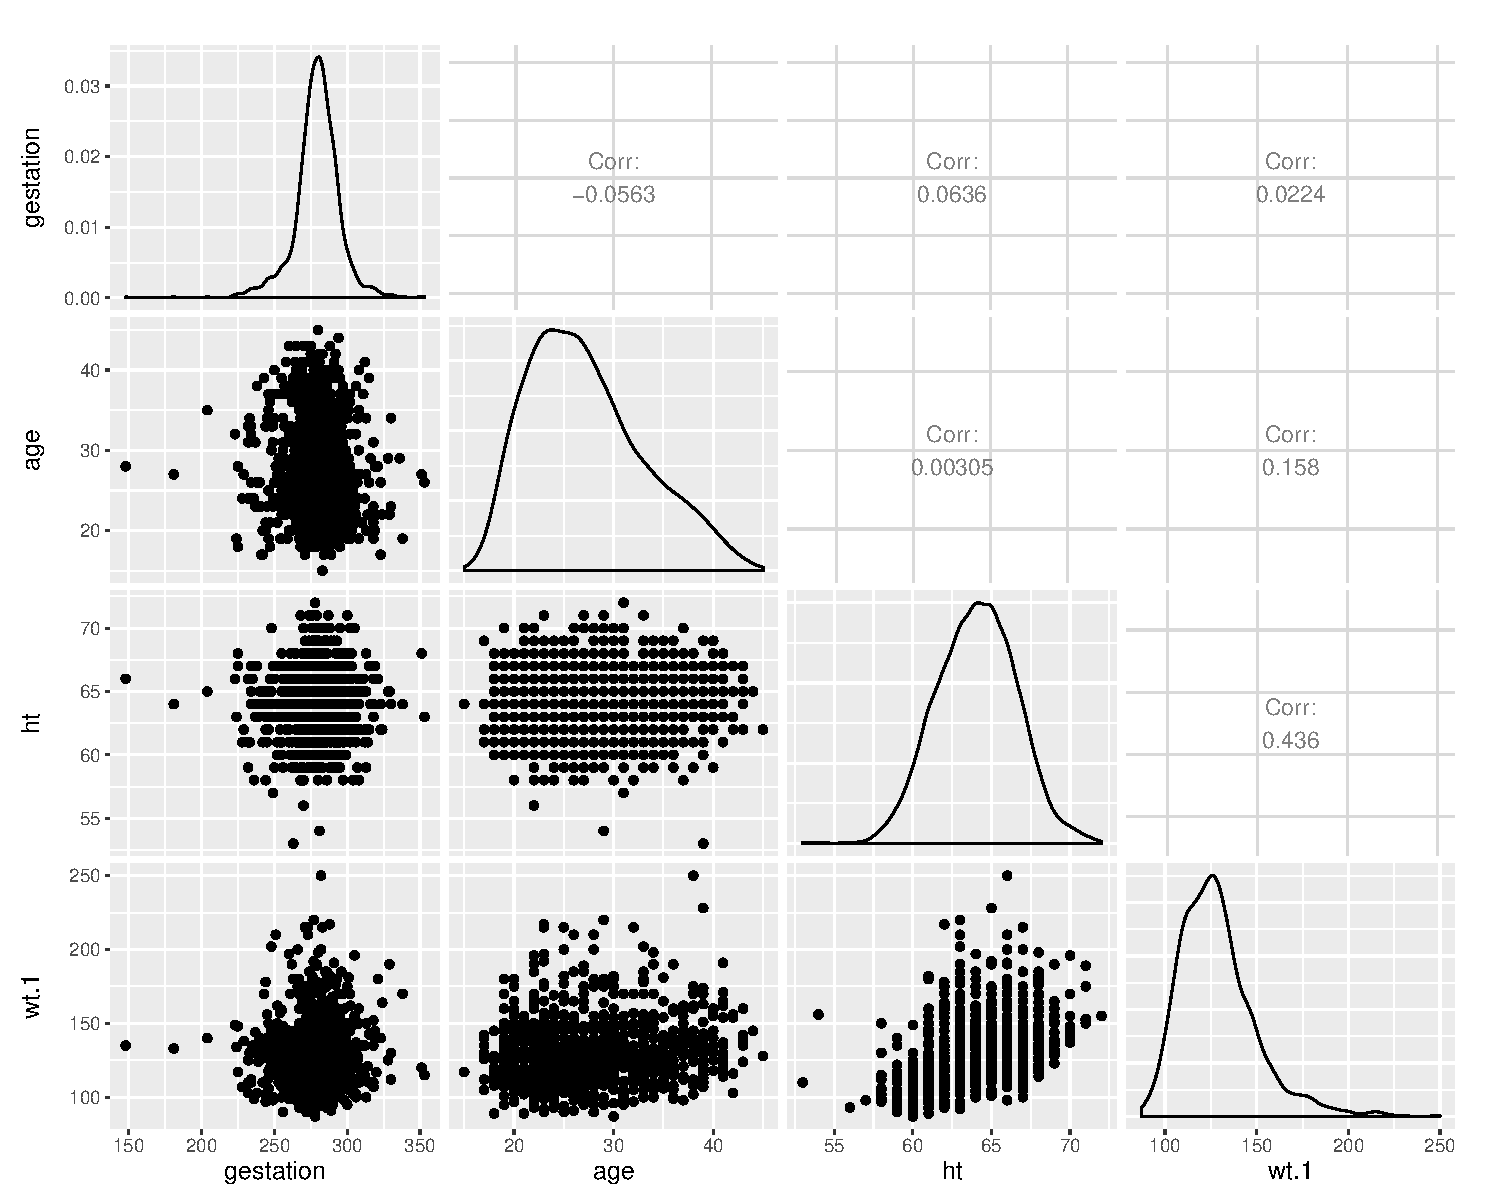
\includegraphics[width=\maxwidth]{figure/unnamed-chunk-8-1} 

\end{knitrout}

However, if $np < 10$ or $n(1-p) < 10$, then the normal approximation is likely not sufficiently good. Suppose that we had only sampled 12 people instead of 123. 


% 
% \paragraph{Exercise: Batting Averages, redux}
% 
% Previously, we considered Ted Williams' batting average of .406 in 1941, which is unmatched in 72 years and counting. In 1994, Tony Gwynn of the San Diego Padres hit .394, but a strike by the player's union shortened the season after only 116 games. Thus, Gwynn accumulated 165 hits in 419 at-bats, whereas Williams had 185 hits in 456 at-bats. Let's assume that Gwynn had an unknown, fixed true batting average of $p$ in 1994. 
% 
% \begin{enumerate}
%   \itemsep1.5in
%   \item The league average batting average in 1994 was .277. Use the normal approximation to test -- at the 5\% level -- the hypothesis that Gwynn was a league-average hitter. Do you reject or fail to reject? (\emph{Hint: If you don't have a computer to compute the p-value, find the $z$-score and approximate using the Empirical Rule})
% 
%   \item Use the normal approximation to find a 95\% confidence interval for Gwynn's true batting average $p$. (\emph{Hint: Be sure to use $\hat{p}$ when computing the standard error! (see page 124)})
%   
%   
%   \item Does the confidence interval that you found contain the hypothesized proportion of .277? Does it contain .400? 
%   
%   \item A sportswriter claims that Gwynn does not deserve to be mentioned in the same breath as Williams, because Williams hit .400, but Gwynn did not. Does your analysis refute or support this claim? 
% 
%   \vspace{1.5in}

%\end{enumerate}







% 
% \newpage
% 
% \paragraph{Solution to Warmup}
% 
% <<message=FALSE>>=
% require(mosaic)
% require(mosaicData)
% favstats(~ gasbill, data=Utilities)
% favstats(~ elecbill, data=Utilities)
% @
% 
% \paragraph{Inference for a Single Proportion}
% 
% 
% 
% \paragraph{Solution to Exercises}
% 
% <<message=FALSE>>=
% require(Lahman)
% players = subset(Batting, yearID == 1994 & AB > 200)
% favstats(~(H/AB), data=players)
% @
% 
% \begin{enumerate}
%   \item 
%   
%   
% <<>>=
% n = 419
% p_hat = 165/419
% p.0 = .277
% se = sqrt(p_0 * (1 - p.0) / n)
% 2 * pnorm(p_hat, mean=p_0, sd=se, lower.tail=FALSE)
% @
% 
%   \item 
% 
% <<>>=
% se = sqrt(p_hat * (1 - p_hat) / n)
% p_hat + c(-1.96, 1.96) * se
% @
% 
% \end{enumerate}
% 
% <<fig.height=4>>=
% g = subset(Batting, playerID == "gwynnto01" & yearID == 1994)
% t = subset(Batting, playerID == "willite01" & yearID == 1941)
% n.g = g[1,"AB"]
% p.g = g[1,"H"] / n.g
% se.g = sqrt(p.g * (1 - p.g) / n.g)
% 
% n.t = t[1,"AB"]
% p.t = t[1,"H"] / n.t
% se.t = sqrt(p.t * (1 - p.t) / n.t)
% 
% d = p.g - p.t
% se = sqrt(se.g^2 + se.t^2)
% d + c(-1.96, 1.96) * se
% xpnorm(d, mean=0, sd = se)
% @
% 

\end{document}
